 \chapter{Modifying Gale Diagrams}\label{chap:GaleDiagMod}

This chapter explores certain operations on Gale diagrams and how these operations affect the polytopes.



\section{Joins and Direct Sums}

Recall, from Sections \ref{SSec:Join} and \ref{SSec:DirectSum}, the definitions of join and direct sum for point sets.  If \(X=\seta{\ve p_1,\ve p_2\dc\ve p_n}\sbset\R{d_1}\) and \(Y=\seta{\ve q_1,\ve q_2\dc\ve q_m}\sbset\R{d_2}\), then
    \[
        X\join Y
            =
                \setb{\begin{bmatrix}\ve p_i\\\ve0_{d_2}\\-1\end{bmatrix}}{i\in\brac n}
                \cup
                \setb{\begin{bmatrix}\ve 0_{d_1}\\\ve q_j\\1\end{bmatrix}}{j\in\brac m}
            \sbset
                \R{d_1+d_2+1}
    \]
and
    \[
        X\oplus Y
            =
                \setb{\begin{bmatrix}\ve p_i\\\ve0_{d_2}\end{bmatrix}}{i\in\brac n}
                \cup
                \setb{\begin{bmatrix}\ve 0_{d_1}\\\ve q_j\end{bmatrix}}{j\in\brac m}
            \sbset
                \R{d_1+d_2}.
    \]
Since these operations are defined for general point sets, it makes sense to ask what happens if you perform them on two Gale diagrams.
\begin{Theorem}\label{Thm:DSumAndJoin}
    If \(P\) and \(Q\) are polytopes, \(\Gamma\in\galed(P)\), and \(\Lambda\in\galed(Q)\), then
        \[
            \Gamma\oplus \Lambda
                \in
                \galed(P\join Q)
        \]
    and
        \[
            \Gamma\join \Lambda
                \in
                \galed(P\oplus Q).
        \]
\end{Theorem}
\begin{proof}
    Suppose the following:
        \begin{align*}
            \dim P&=d_1;&
                \dim Q&=d_2;\\
            P&\sbset\R{d_1};&
                Q&\sbset\R{d_2};\\
            \vrt P&=\seta{\ve v_1,\ve v_2\dc\ve v_n};&
                \vrt Q&=\seta{\ve w_1,\ve w_2\dc\ve w_m};\\
            \ve 0_{d_1}&\in\relint P;&
                \ve 0_{d_2}&\in\relint Q;\\
            \dim\aff&\seta{\ve v_1,\ve v_2\dc\ve v_{d_1+1}}=d_1;&
                \dim\aff&\seta{\ve w_1,\ve w_2\dc\ve w_{d_2+1}}=d_2;
        \end{align*}
    and
        \begin{align*}
            \rref
                    \begin{bmatrix}
                        1       &   1       &   \cdots  &   1       \\
                        \ve v_1 &   \ve v_2 &   \cdots  &   \ve v_n
                    \end{bmatrix}
                        &=
                        \left[
                            \begin{array}{@{}c|c@{}}
                                I_{d_1+1} & A
                            \end{array}
                        \right]; &
                \rref
                    \begin{bmatrix}
                        1       &   1       &   \cdots  &   1       \\
                        \ve w_1 &   \ve w_2 &   \cdots  &   \ve w_m
                    \end{bmatrix}
                        &=
                        \left[
                            \begin{array}{@{}c|c@{}}
                                I_{d_2+1} & B
                            \end{array}
                        \right].
        \end{align*}
    Then order the vertices of \(P\join Q\) as follows:
        \begin{align*}
                \seta{
                \begin{bmatrix} \ve v_1\\       \ve 0_{d_2}\\   -1  \end{bmatrix}\dc
                \begin{bmatrix} \ve v_{d_1+1}\\ \ve 0_{d_2}\\   -1  \end{bmatrix},
                \begin{bmatrix} \ve 0_{d_1}\\   \ve w_1 \\      1   \end{bmatrix}\dc
                \begin{bmatrix} \ve 0_{d_1}\\   \ve w_{d_2+1}\\ 1   \end{bmatrix},
                \begin{bmatrix} \ve v_{d_1+2}\\ \ve 0_{d_2}\\   -1  \end{bmatrix}\dc
                \begin{bmatrix} \ve v_{n}\\     \ve 0_{d_2}\\   -1  \end{bmatrix},
                \begin{bmatrix} \ve 0_{d_1}\\   \ve w_{d_2+2}\\ 1   \end{bmatrix}\dc
                \begin{bmatrix} \ve 0_{d_1}\\   \ve w_{m}\\     1   \end{bmatrix}
                }.
        \end{align*}
    Here, the first \(d_1+d_2+2=\dim(P\join Q)+1\) vertices are affinely independent.  Now, use the techniques of Section \ref{SSec:ComputingGD} to compute a Gale transformation of \(P\join Q\) as follows:
    Form the matrix
        \begin{align*}
            Z=
            \left[
            \begin{array}{ccc|ccc|ccc|ccc}
                1               &\cdots  &1               &1               &\cdots  &1
                &1              &\cdots  &1               &1               &\cdots  &1   \\
                \ve v_1         &\cdots  &\ve v_{d_1+1}   &\ve 0_{d_1}     &\cdots  &\ve 0_{d_1}
                &\ve v_{d_1+2}  &\cdots  &\ve v_n         &\ve 0_{d_1}     &\cdots  &\ve 0_{d_1}     \\\hline
                \ve 0_{d_2}     &\cdots  &\ve 0_{d_2}     &\ve w_1         &\cdots  &\ve w_{d_2+1}
                &\ve 0_{d_2}    &\cdots  &\ve 0_{d_2}     &\ve w_{d_2+1}   &\cdots  &\ve w_m         \\
                -1              &\cdots  &-1              &1               &\cdots  &1
                &-1             &\cdots  &-1              &1               &\cdots  &1
            \end{array}
            \right].
        \end{align*}


    First, add the first row to the last row, and then perform, in the first \(d_1+1\) rows, the operations that transformation the matrix \(\left[\begin{array}{cccc}1&1&\cdots&1\\ \ve v_1&\ve v_2&\cdots&\ve v_n\end{array}\right]\) into \(\left[\begin{array}{@{}c|c@{}}I_{d_1+1} & A\end{array}\right]\).  Note that in the \(1,2\) and \(1,4\) blocks each column will be the same.  Call this common \((d_1+1)\)-dimensional vector \(\ve v\).  Further, denote an \(r\times s\) matrix with all entries \(0\) by \(\zmat rs\).  That is,
            \begin{comment}
            \rref\left[
                \begin{array}{ccc|ccc|ccc|ccc}
                    1               &\cdots     &1
                    &1              &\cdots     &1
                    &1              &\cdots     &1
                    &1              &\cdots     &1
                    \\
                    \ve v_1         &\cdots     &\ve v_{d_1+1}
                    &\ve0_{d_1}     &\cdots     &\ve0_{d_1}
                    &\ve v_{d_1+2}  &\cdots     &\ve v_n
                    &\ve0_{d_1}     &\cdots     &\ve0_{d_1}
                    \\  \hline
                    \ve 0_{d_2}     &\cdots     &\ve 0_{d_2}
                    &\ve w_1        &\cdots     &\ve w_{d_2+1}
                    &\ve0_{d_2}     &\cdots     &\ve 0_{d_2}
                    &\ve w_{d_2+2}  &\cdots     &\ve w_{m}
                    \\
                    -1              &\cdots     &-1
                    &1              &\cdots     &1
                    &-1             &\cdots     &-1
                    &1              &\cdots     &1
                \end{array}
            \right]\\
            \end{comment}
        \begin{align*}
            M&= \rref Z
                =
                \rref\left[
                    \begin{array}{c|c|c|c}
                        I_{d_1+1}
                            &\begin{array}{ccc}{\olay{\ve v}{\ve w_1}}&\cdots&{\olay{\ve v}{\ve w_{d_2+1}}}\end{array}
                            &A
                            &\begin{array}{ccc}\olay{\ve v}{\ve w_{d_2+2}}&\cdots&\olay{\ve v}{\ve w_m}\end{array}
                        \\ \hline
                        \zmat{d_2+1}{d_1+1}
                            &\begin{array}{ccc}\ve w_1&\cdots&\ve w_{d_2+1}\\ 2&\cdots&2\end{array}
                            &\zmat{d_2+1}{n-d_1+1}
                            &\begin{array}{ccc}\ve w_{d_2+2}&\cdots&\ve w_{m}\\ 2&\cdots&2\end{array}
                    \end{array}
                \right].
        \end{align*}

    Next, use the bottom row of the matrix to turn the \(1,2\) and \(1,4\) blocks into all zeros.  Then move the bottom row to the \((d_1+2)\)th row, divide it by \(2\) and shift each of the remaining rows down, that is:
        \begin{align*}
            M
                &=
                \rref\left[
                    \begin{array}{c|c|c|c}
                        I_{d_1+1}
                            &\zmat{d_1+1}{d_2+1}
                            &A
                            &\zmat{d_1+1}{m-d_2-1}
                        \\ \hline
                        \zmat{d_2+1}{d_1+1}
                            &\begin{array}{ccc}1&\cdots&1\\ \ve w_1&\cdots&\ve w_{d_2+1}\end{array}
                            &\zmat{d_2+1}{n-d_1+1}
                            &\begin{array}{ccc}1&\cdots&1\\ \ve w_{d_2+2}&\cdots&\ve w_{m}\end{array}
                    \end{array}
                \right].
        \end{align*}

    Now, in the bottom \(d_2+1\) rows, perform the row operations that transformation the matrix \(\left[\begin{array}{cccc}1&1&\cdots&1\\ \ve w_1&\ve w_2&\cdots&\ve w_m\end{array}\right]\) into \(\left[\begin{array}{@{}c|c@{}}I_{d_2+1} & B\end{array}\right]\).  Thus
        \begin{align*}
            M
                &=
                \left[
                    \begin{array}{c|c}
                        I_{d_1+d_2+2}
                            &\hspace{-5pt}\begin{array}{c|c}
                                A   &[0]\\
                                \hline
                                [0] &B
                             \end{array}
                    \end{array}\hspace{-5pt}
                \right]
        \end{align*}
    and so a Gale transformation of \(P\join Q\) is given by the multiset of the columns of the matrix
        \begin{align*}
            \left[
                \begin{array}{c|c|c|c}
                    -\Tr A  &[0]    &I      &[0]    \\ \hline
                    [0]     &-\Tr B &[0]    &I
                \end{array}
            \right].
        \end{align*}
    These are exactly the elements of \(\Gamma\oplus\Lambda\).

    The second result holds by oriented matroid duality.
\end{proof}


\subsection{\protect$d\protect$-Polytopes with \protect$d+2\protect$ Vertices}\label{SSec:dPlusTwo}
    As an application of Theorem \ref{Thm:DSumAndJoin}, all \(d\)-polytopes with \(d+2\) vertices are classified.  This section follows the discussion found in \cite{McMullenBook}.

    Let \(P\) be a \(d\)-polytope with \(d+2\) vertices, and let \(\Gamma\) be a standard Gale diagram of \(P\).  Since \(\Sp0=\seta{-1,1}\sbset\RR\), as a set \(\seta{-1,1}\sbset\Gamma\sbset\seta{-1,0,1}\).  Because \(\Gamma\) is a Gale diagram,
        \begin{align*}
            p
                &=  \card{\setb{\ve x\in\Gamma}{\ol{\ve x}=-1}}
                    \ge 2\\
            q
                &=  \card{\setb{\ve x\in\Gamma}{\ol{\ve x}=1}}
                    \ge 2.
        \end{align*}
    This leaves \(a=d+2-p-q\) points in \(\Gamma\), and they must all be at the origin.  A point at the origin in a Gale diagram corresponds to the apex of a pyramid in the polytope (Theorem \ref{Thm:GalePyr}).  Thus \(P\) is an \(a\)-fold pyramid over a polytope \(Q\) whose Gale diagram \(\Lambda\) has \(p\ge 2\) points on one side of the origin, and \(q\ge 2\) points on the other.

    The Gale diagram \(\Lambda\) is the join of the Gale diagrams of a \((p-1)\)-simplex and a \((q-1)\)-simplex.  Hence, by Theorem \ref{Thm:DSumAndJoin}, \(P\) is combinatorially equivalent to the polytope
        \[
            \pyr_a\left(\simp{p-1}\oplus\simp{q-1}\right).
        \]
    where \(a+p+q=d+2\) and \(p,q\ge 2\).

    Note that the combinatorial type of each \(d\)-polytope with \(d+2\) vertices can be specified by the unordered pair \((p,q)\).  So to count the number of combinatorial types of these polytopes, one only needs to count the number of such pairs.  Assume, without loss of generality, that \(p\le q\).  The pairs are then of the following form:
        \begin{align*}
            (2,q)
                &,\qquad 2\le q\le d\\
            (3,q)
                &,\qquad 3\le q\le d-1\\
                &\vdots\\
            \left(\floor{\frac d2},q\right)
                &,\qquad \floor{\frac d2}\le q\le\ceil{\frac d2}.
        \end{align*}

    Thus, if \(d\) is odd, then there are
        \begin{align*}
            2+4+\dotsb+(d-1)
                &=  2\left(1+2+\dotsb+\frac{d-1}2\right)
                =   \frac{d^2}4-\frac14
                =   \floor{\frac{d^2}4}
        \end{align*}
    combinatorial types of these polytopes.  If \(d\) is even, then there are
        \begin{align*}
            1+3+\dotsb+(d-1)
                &=  2+4+\dotsb+d-\frac d2
                =   \frac{d^2}4
                =   \floor{\frac{d^2}4}
        \end{align*}
    types of these polytopes.

    In \cite{McMullenBook}, the following lemma is proved.
    \begin{Lemma}
        Let \(\Gamma\) be a Gale diagram of a \(d\)-polytope \(P\) with \(n\) vertices.  Then \(P\) is a simplicial polytope if and only if for every hyperplane \(H\in\R{n-d-1}\) containing \(\ve 0\) the following holds:
            \[
                \ve 0
                    \notin \relint\conv(\Gamma\cap H).
            \]
    \end{Lemma}

    Combining this with the above discussion yields:
    \begin{Theorem}
        There are \(\floor{{d^2}/4}\) combinatorial types of \(d\)-polytopes with \(d+2\) vertices.  Furthermore, each of these polytopes is of the form \(\pyr_a\left(\simp{p-1}\oplus\simp{q-1}\right)\) where \(a+p+q=d+2\) and \(p,q\ge2\).  Moreover, \(\floor{d/2}\) of these polytopes are simplicial.
    \end{Theorem}

    \begin{comment}
    Thus, letting \(\Gamma(\simp{j})\) denote the standard Gale diagram of the \(j\)-simplex,
         \[
            \Gamma  =   \Gamma(\simp{k_{-1}-1})\join\Gamma(\simp{k_{1}-1}).
         \]
    Hence, by Theorem \ref{Thm:DSumAndJoin}, \(P\) is a direct sum of two simplices.
    \end{comment}

\section{Adding Points to Gale Diagrams}
    The first thing one should do in a section entitled ``Adding Points to Gale Diagrams" is discuss under what conditions adding a point to a Gale diagram yields a Gale diagram.  Thus, suppose \(\Gamma\in\galed(P)\) is a Gale diagram of some \(d\)-polytope \(P\) with \(n\) vertices, and let \(\ve x\in\R{n-d-1}\) be any point.  Then \(\Gamma\cup\seta{\ve x}\) is a Gale diagram of some \((d+1)\)-polytope with \(n+1\) vertices.  This is true since every hyperplane still has at least two points in both of its open half-spaces.  It should be clear that the location of the new point does matter in determining the new polytope.  Adding a point to a Gale diagram increases the number of points by \(1\), but not the dimension of the space in which the Gale diagram lies. Thus the dimension of the new polytope is \(1\) greater than the dimension of the old polytope.

    Points can be added to Gale diagrams in many ways.  Unfortunately, it is possible given two Gale diagrams  \(\Gamma,\Lambda\in\galed(P)\) to add a point to both \(\Gamma\) and \(\Lambda\) in the same way (such as adding a point antipodal to the point corresponding to a particular vertex), yet not have the two new polytopes be combinatorially equivalent.

    \subsection{Adding an Antipode to a Gale Diagram}
        \begin{figure}[p!hbt]
            \centering
                \includegraphics[width=.7\textwidth, page=16]{pictures.pdf}
            \caption{Two Gale diagrams of $\xp3$.\label{Fig:2GaleDXp3}}
        \end{figure}

        \begin{figure}[p!hbt]
            \centering
                \includegraphics[width=.8\textwidth, page=17]{pictures.pdf}
            \caption{Adding an antipode $\ol{1'}$ to the point $\ol{1}$ in a Gale diagram of $\xp3$. (cf.{} Figure \ref{Fig:AddPt2Gale2})\label{Fig:AddPt2Gale1}}
        \end{figure}

        \begin{figure}[p!hbt]
            \centering
                \includegraphics[width=.8\textwidth, page=18]{pictures.pdf}
            \caption{Adding an antipode $\ol{1'}$ to the point $\ol{1}$ in a Gale diagram of $\xp3$. (cf.{} Figure \ref{Fig:AddPt2Gale1})\label{Fig:AddPt2Gale2}}
        \end{figure}

        As an example; consider the crosspolytope \(\xp3\).  Figure \ref{Fig:2GaleDXp3} shows two consubstantial standard Gale diagrams for \(\xp3\).  If a point \(\ol{1'}\) is added that is antipodal to \(\ol 1\) in each of these Gale diagrams, then Figures \ref{Fig:AddPt2Gale1} and \ref{Fig:AddPt2Gale2} show the graphs of the polytopes with each of these Gale diagrams.  Let \(P\) be a polytope with the Gale diagram in Figure \ref{Fig:AddPt2Gale1}, and \(Q\) be a polytope with the Gale diagram in Figure \ref{Fig:AddPt2Gale2}.  Note that \(\conv\seta{2,5}\) is not an edge in \(P\), whereas in \(Q\) it is.  Hence, \(P\) and \(Q\) cannot be combinatorially equivalent.

        The facets of \(P\) are the \(3\)-dimensional pyramids \(23456\) and \(12345\) each with base \(2345\), as well as the following \(3\)-simplices.
            \begin{align*}
                &11'45&     &11'35&     &11'24&     &11'23\\
                &1'456&     &1'356&     &1'246&     &1'236
            \end{align*}
        The facets of \(Q\) are the triangular bipyramid \(23456\) with base \(256\), as well as the following \(3\)-simplices.
            \begin{align*}
                &11'45&     &11'35&     &11'24&     &11'23\\
                &1'456&     &1'356&     &1'246&     &1'236\\
                &1245&      &1235&      &&&
            \end{align*}
    \subsection{Duplicating a Point in a Gale Diagram}
        On the other hand, an operation that is well defined is that of adding a duplicate of an existing point to a Gale diagram.
        Let \(P\) be a \(d\)-polytope with vertex set \(\vrt P=\seta{\ve v_1,\ve v_2\dc\ve v_n}\).  Let \(\Gamma\) be a Gale diagram of \(P\), and let \(Q\) be a \((d+1)\)-polytope with vertex set \(\vrt Q=\seta{\ve w_{1'},\ve w_1,\ve w_2\dc\ve w_n}\) whose Gale diagram \(\Lambda\) satisfies \(\ol{\ve w}_{1'}=\ol{\ve v}_1\) and \(\ol{\ve w}_i=\ol{\ve v}_i\) otherwise.

        Let \(Y\) be a cofacet of \(Q\), that is, a minimal coface and consider the following four cases:
            \begin{enumerate}
                \item   (\(\seta{\ve w_1,\ve w_{1'}}\sbset Y\))  This case cannot happen since the set \(\ol{Y}\setminus\seta{\ol{\ve w}_1}\) captures the origin, and \(Y\setminus\seta{\ve w_1}\varsubsetneq Y\).
                \item   (\(\ve w_1\in Y\) and \(\ve w_{1'}\notin Y\))  For this case, let \(X=\setb{\ve v_i}{\ve w_i\in Y}\).  Then since \(\ol Y=\ol X\), the set \(Y\) is a cofacet if and only if \(X\) is a cofacet.
                \item   (\(\ve w_1\notin Y\) and \(\ve w_{1'}\in Y\))  Here, set \(X=\setb{\ve v_i}{\ve w_i\in Y\text{ or }i=1}\).  In this case, \(\ol Y=\ol X\) again, and so \(Y\) is a cofacet if and only if \(X\) is a cofacet.
                \item   (\(\seta{\ve w_1,\ve w_{1'}}\cap Y=\mt\)) For the final case, again set \(X=\setb{\ve v_i}{\ve w_i\in Y}\).  Once more, \(\ol Y=\ol X\), so that \(Y\) is a cofacet if and only if \(X\) is a cofacet.
            \end{enumerate}
        Thus the cofacets (and hence the facets) of \(Q\) are determined by the cofacets (and hence the cofacets) of \(P\) and vice versa. Geometrically, \(Q\) is combinatorially equivalent to a polytope with the following vertices:
            \begin{align*}
                \ve w_1
                    &=   \begin{bmatrix}\ve v_1\\1 \end{bmatrix}&
                \ve w_{1'}
                    &=   \begin{bmatrix}\ve v_1\\-1 \end{bmatrix}&
                \ve w_j
                    &=   \begin{bmatrix}\ve v_j\\0 \end{bmatrix},\,j\in\brac n\setminus\seta1
            \end{align*}
        Conceptually, first place \(P\) in \(\R{d+1}\).  Then the vertex \(\ve v_1\) is replaced by a line segment whose relative interior passes through \(\ve v_1\), and whose affine hull intersects that of the original polytope at precisely the point \(\ve v_1\).

        If \(P\) is a \(2\)-polytope with \(n\) vertices, then performing this operation at any vertex yields a polytope that is combinatorially equivalent to performing the operation at any other vertex.  The resulting polytope is combinatorially equivalent to the cyclic polytope \(\cyc{n+1}3\).  See Figure \ref{Fig:DupGale} for an example.  This process is called a \dfn{simplicial wedge} in \cite{SimplicialWedge}.

        \begin{figure}[p!hbt]
            \centering
                \includegraphics[width=.7\textwidth, page=32]{pictures.pdf}
            \caption{Duplicating the point\protect$\ol1\protect$ in a Gale diagram of \protect$\cyc25\protect$.\label{Fig:DupGale}}
        \end{figure} 